\documentclass[11pt]{article}
\usepackage{amsmath}
\usepackage{graphicx}
\setlength{\oddsidemargin}{0.0in}
\setlength{\evensidemargin}{0.0in}
\setlength{\topmargin}{-0.25in}
\setlength{\headheight}{0in}
\setlength{\headsep}{0in}
\setlength{\textwidth}{6.5in}
\setlength{\textheight}{9.25in}
\setlength{\parindent}{4em}
\setlength{\parskip}{2mm}

\begin{document}

\noindent{\textbf{\LARGE{Introduction}}}\\ \\
\noindent{\textbf{\large{Database \(train.csv\)}}}\\

\par
	In section B of the term project we were given a data set of Porto taxi trips \(train.csv\).
 The dataset was based off of 442 Taxises in the city of Porto, Portugal. The data was split among 9
 categories TRIP\_ID, CALL\_TYPE, ORIGIN\_CALL, ORIGIN\_STAND, TAXI\_ID, TIMESTAMP, DAYTYPE, MISSING\_DATA,
 POLYTIME and consisted of 1710660 objects sized at 1.94 GB. The TRIP\_ID was a unique identifier for
every trip and TAXI\_ID was a unique identifier for the taxi driver who performed the trip. CALL\_TYPE
 identified the method used to call the taxi: \textsc{\char13}A\textsc{\char13} represented a call from central,
 \textsc{\char13}B\textsc{\char13} represented if the taxi driver was demanded at a specific stand, and 
\textsc{\char13}C\textsc{\char13} otherwise. ORIGIN\_CALL represented the phone number of the customer who
 demanded the taxi $($ Sets CALL\_TYPE to \textsc{\char13}A\textsc{\char13}$)$. ORIGIN\_STAND gives each taxi
 stand a unique identifier $($Sets CALL\_TYPE to \textsc{\char13}B\textsc{\char13}$)$ .TIMESTAMP shows the unix
 Timestamp of the start of the trip. DAYTYPE represents the type of day it is at the start of the trip: \textsc{\char13}B
\textsc{\char13} being a holiday or special day, \textsc{\char13}C\textsc{\char13} being the day before a type
 \textsc{\char13}B\textsc{\char13} day, and \textsc{\char13}A\textsc{\char13} being everything else.Lastly,
 POLYLINE contains a set of arrays of two elements of global coordination, the longitude and latitude.\\

\noindent{\textbf{\large{Dealing with a massive dataset}}}\\
\par
	 In order to use the dataset, we had to import it into our R data table which at first we did by using the read$()$
 function. This created an issue because the data set was taking too long to load in and often times crashing the
 IDE due to insufficient memory. A temporary fix we decided to use was to only pass in 1000 rows of the full data 
set. This allowed us to get past the issues of read$()$ and start working on the tasks in part B. In order to fully
 fix this problem and use the entire data set we decided to use fread$()$from the data.table library. This allowed
 us to read the data set faster and use less memory.\\

\noindent{\textbf{\large{Tasks to solve}}}\\
\begin{itemize}
	\item Find density models that accurately represented the trip duration and the time when the driver was busy.
	\item Explore if the CALL\_TYPE had an effect on the meantime of taxi trips
	\item Create models that predicted trip times, distances, …$($Add other explicit models$)$
	\item Compare how those predictive models relate to one another.
\end{itemize}

\noindent{\textbf{\large{Language and Libraries used}}}\\
\par To solve these tasks our group used R to code the entire project as specified in the instructions.
 We also used the following libraries throughout the project

\begin{itemize}
	\item Devtools: Used to assist in the installation of Regtools later in the project.
	\item Dplyr: Utilized this library to create and edit data frames.
	\item Data.table: Primarily used for fread$()$ in order to speed up reading of \(train.csv\).
	\item Regtools: Allowed us to utilize many machine learning models
\end{itemize}

\noindent{\textbf{\LARGE{Exploring the possibility of trip duration}}}\\ \\
\noindent{\textbf{\large{The trip duration in this database}}}\\
\par
Since POLYLINE represents a set of coordinates recorded every fifteen seconds since the start of the trip,
 The duration of a trip can be interpreted as the number of intervals existing in the set. In terms of calculation,
 letting $N_i$ donates to the number of intervals in $i^{th}$ set, The duration of $i^{th}$ trip in second is
\begin{equation}
T_i = 15(N_i -1)
\end{equation}
\par
To be more general, we convert the duration into minutes by dividing it by 60.

\noindent{\textbf{\large{The probability family of distribution of trip duration:}}}\\
\par
Now we have a column called trip duration, so we use hist to plot the trip duration into an histogram with the x axis as the trip duration and the y axis as the density. The probability of trip duration is found to be a gamma distribution family in the interval [0, 970], but because most of time is distributed within the starting proportion , which makes the original histogram hard to be observed, we shrink the range of x axis to [0, 100]. However, the gamma distribution seems to only exist in [1,100] because the probability that the trip time is under a minute is too high too fit into the gamma distribution.

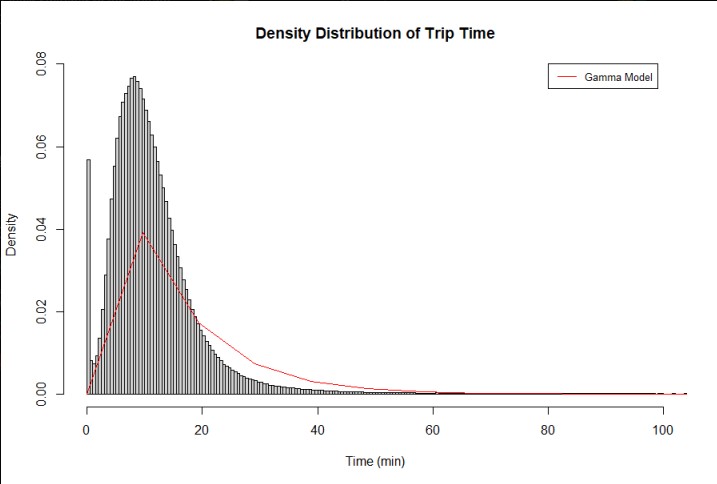
\includegraphics[scale = .75]{DensityDistTripTime.png}

\noindent{\textbf{\large{Verify the hypothesis:}}}
\par
To test whether the probability density of trip duration is the gamma family of distribution, we apply the actual curve of gamma distribution. Therefore, we need to find the r and lambda value, which are found to be 1.0947 and 0.0917.

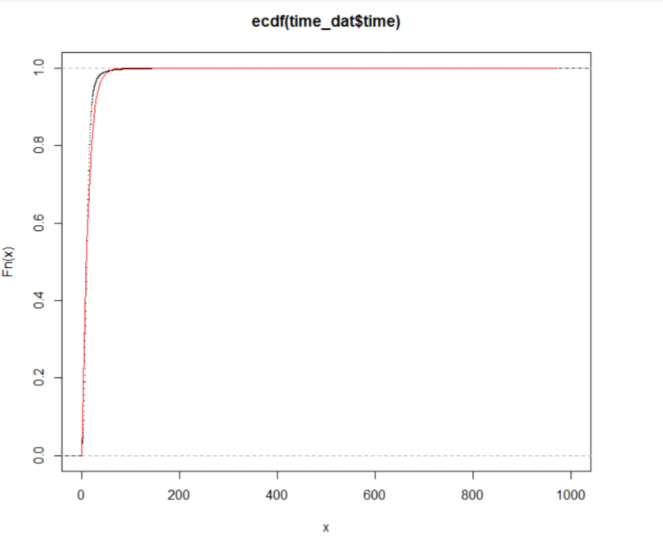
\includegraphics[scale = .75]{ECDF(time_dat$time).png}

\par
We also compare empirical cdf of T and cdf of gamma distribution with r and lambda which we just found. However, they don’t match well 

\noindent{\textbf{\large{Exploring the distribution of proportion of driver is busy:}}}\\\\
\textbf{Definition of Busy:}

\par
Literally, drivers being busy means they are working, but in order to calculate the proportion of drivers being busy, we also need to know when they are not busy, waiting for passengers or including they time are are off work, We assume that taxi drivers don’t have specifical time to work and amount of operating time, so we decide to define the total time as ones career life recorded in the database, from the beginning of a driver’s first trip to the ending time of his last trip. Since each driver has an unique id number, we can track the sum of trip duration as the total working time 
of $i^{th}$ driver, denoting as $U_{i}$, and Let $T_i$ denotes to the total time of $i^{th}$ driver, $R_{i_j}$ denotes to the $j^{th}$ trip duration of the $i^{th}$ driver, $N_i$ denotes to the number of trips $i^{th}$ driver have completed, and $B_i$ denotes to the proportion of time $i^{th}$ driver being busy; the time can be calculated as

\begin{equation}
T_i =TimeStamp_{i last}-TimeStamp_{i first} +R_{iN_i}
\end{equation}

\par
The busy time is as

\begin{equation}
U_i = \sum_{k=1}^{N_i} R_{ik}
\end{equation}

\par
Then, the proportion is

\begin{equation}
B_i = \frac{U_i}{T_i}
\end{equation}

\textbf{Probability Distribution:}
\par
Plotting B into the histogram, we get an approximate normal distribution in the range of (0,0.23]. As we observe there are some extreme cases that drivers only work about 0.005 of their time involved in this career, averagely 0.12 hour a day.

\noindent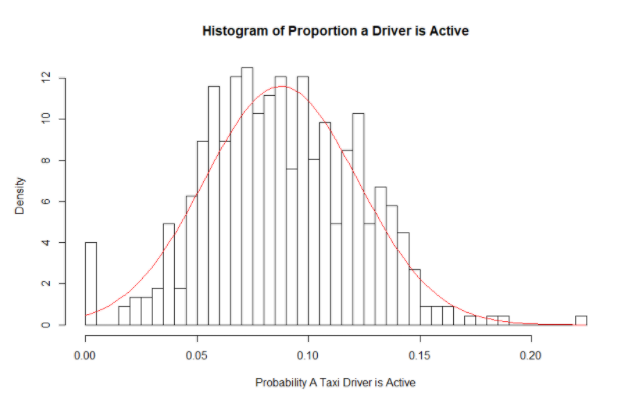
\includegraphics{Hist(PropActDriv).png}\\

\noindent{\textbf{\LARGE{Investigation of average trip times using CALLTYPE:}}}
\centering\noindent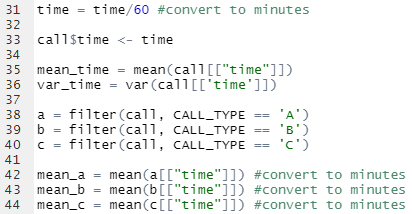
\includegraphics{Part3(Code).png}\\

\flushleft\par
The trip times used in the data set have been given in terms of UNIX timestamps which make it hard to visualize. In order to get a better understanding of trip times, we decided to convert the timestamps into minutes using the following conversion rates:

\begin{itemize}
	\item One minute = 60 UNIX units
	\item One hour = 3,600 UNIX units
	\item One day = 86,400 UNIX unit
\end{itemize}

\par
The equation to get minutes from UNIX timestamp:

\begin{equation}
Minutes = \frac{UNIX TIMESTAMP}{60}
\end{equation}

\par
After we simply applied the mean() and var() functions to the newly converted TIMESTAMP variable to obtain the mean and variance

\par
General Dataset Mean (TIMESTAMP):

\begin{equation}
Mean (Overall) = \frac{Minutes (Converted)}{1710670} = 11.940
\end{equation}

\par
On the other hand, to get the values with the dependency of CALLTYPE, we used filter() to sort through the data in order to get the correct TIMESTAMP values in regard to the three CALLTYPE’s A,B, and C. After we used mean() to get a mean of the TIMESTAMPS sorted by CALLTYPE. 

\begin{equation}
Mean (CALLTYPE = A) = \frac{Minutes (Converted)}{1710670} = 12.506
\end{equation}

\begin{equation}
Mean (CALLTYPE = B) = \frac{Minutes (Converted)}{1710670} = 11.086
\end{equation}

\begin{equation}
Mean (CALLTYPE = C) = \frac{Minutes (Converted)}{1710670} = 12.873
\end{equation}

\noindent{\textbf{\large{Analysis: }}}
\par
Difference between trip times using different call types:

\begin{equation}
Call Type A = 11.940 - 12.506 = -0.566 (33.96 Seconds Slower)
\end{equation}

\begin{equation}
Call Type B = 11.940 - 11.086 = 0.854(51.24 Seconds Faster)
\end{equation}

\begin{equation}
Call Type C = 11.940 - 12.873 = -0.933 (55.98 Seconds Slower)
\end{equation}

\begin{equation}
Call Type B >Call Type A > Call Type C
\end{equation}

\par
In general, the type of call made to summon a taxi doesn’t make much of a difference in regards to trip time, but the fastest would be from a specific stand. Furthermore, we can examine the variance of each call type to determine the spread of the data set compared to the mean.

\begin{equation}
Variance (Overall) = 130.24
\end{equation}

\begin{equation}
Variance (Call Type A) = 72.26
\end{equation}

\begin{equation}
Variance (Call Type B) = 64.76
\end{equation}

\begin{equation}
Variance (Call Type C) = 269.50
\end{equation}

\par
The Variance of the 3 Call Types are fairly close with the exception of Call Type C. This indicates that there is a lot of volatility in the trip times for Call Type C. This could be caused by the fact that Call Type C takes riders from various methods instead of a set way of getting riders.

\end{document}